\subsection{Prima misura delle particelle alfa}
\FloatBarrier
Sono stati settati gli strumenti, a pressione 600 $mb$.
Si è mantenuto lo Shaping Time a 0.25-0.5 $\mu s$, dopo aver osservato il comportamento. %dire cosa succede
E' stata regolata l'amplificazione in modo da mantenere il picco attorno ai $3V$.
E' stato impostato il trigger in modo tale che fosse circa a metà altezza del picco sull'oscilloscopio. 

%Avevamo visto che a 1,5 V dovevamo impostare circa 96 nel trigger in binario, ma poi, non ricordo per che motivo, abbiamo alzato a 128 tipo

Si è verificato che il numero di segnali spuri fosse inferiore al $30 \%$ del totale, facendo il grafico dei picchi e calcolando l'integrale dei segnali a bassa energia.

E' stato quindi acquisito il primo set di dati (circa 3000 eventi)

\begin{grafico}
 \centering
 \resizebox{\textwidth}{!}{%
 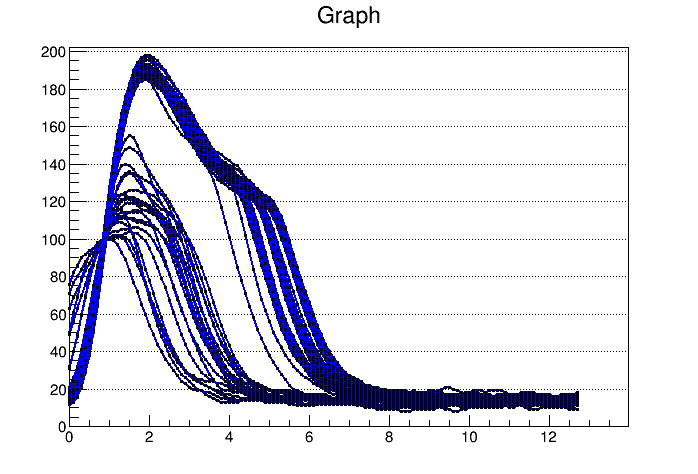
\includegraphics{../grafici/risultati/misura600.png}
 }%
 \caption{Grafico segnali a 600mb in funzione del tempo ($\mu$ s)} 
 \label{gr:misura_600} 
\end{grafico}


E' stato acquisito anche un set di dati con meno eventi e un trigger molto più basso per stimare la baseline.

\begin{grafico}
 \centering
 \resizebox{\textwidth}{!}{%
 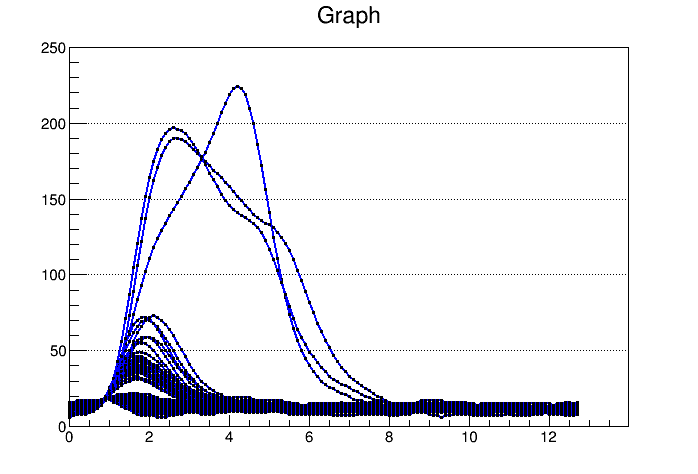
\includegraphics{../grafici/risultati/misura600fondo.png}
 }%
 \caption{Grafico segnali baseline in funzione del tempo ($\mu$ s)} 
 \label{gr:misura600fondo} 
\end{grafico}

E' stato fatto il grafico degli integrali a partire dal file a basso trigger, dove si è visto un picco a bassa energia, corrispondente agli eventi di fondo, e selezionando questi eventi è stato disegnato un istogramma della varibile baseline, da cui calcolando il centroide del picco principale, è stato ricavato il valore da inserire nella macro al posto del valore di default.

\begin{grafico}
 \centering
 \resizebox{\textwidth}{!}{%
 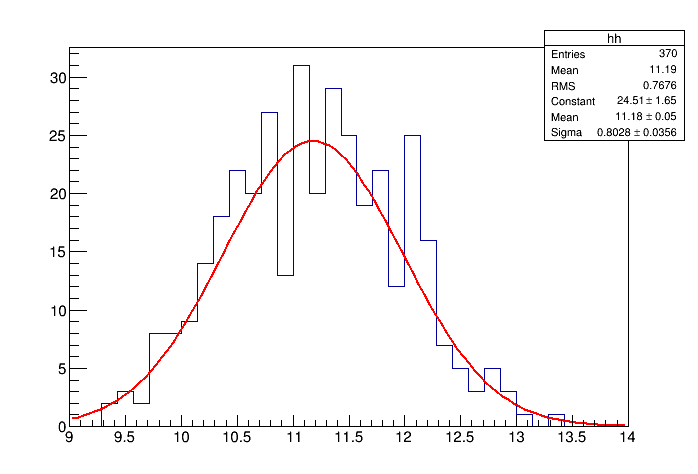
\includegraphics{../grafici/risultati/misura600fondo_baseline.png}
 }%
 \caption{Picco della baseline} 
 \label{gr:misura600fondo_baseline} 
\end{grafico}
%dati baseline

L'analisi dei dati che segue è stata effettuata utilizzando la macro fornite dal laboratorio,
modificando il limite dei campioni da integrare e inserendo il valore della baseline appena stimato.
Il limite dei campioni a 600 mb è stato posto uguale a 90.

\begin{grafico}
 \centering
 \resizebox{\textwidth}{!}{%
 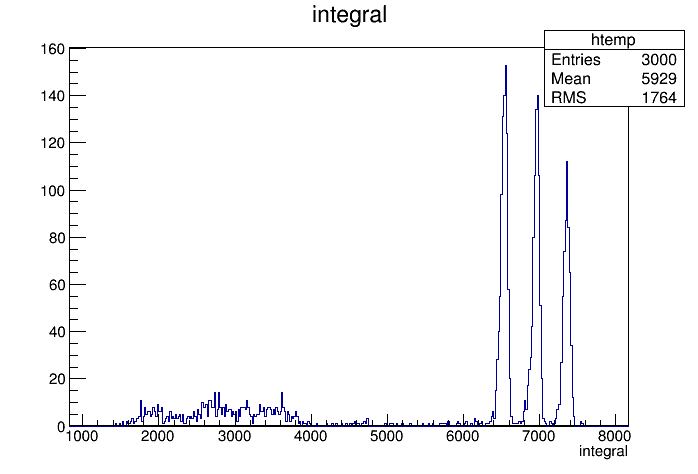
\includegraphics{../grafici/risultati/misura600_integral.png}
 }%
 \caption{Grafico integral} 
 \label{gr:misura600_integral} 
\end{grafico}

 \begin{grafico}
 \centering
 \resizebox{\textwidth}{!}{%
 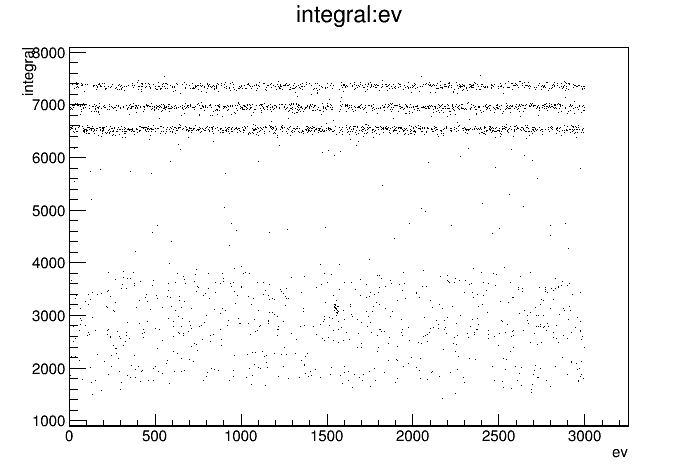
\includegraphics{../grafici/risultati/misura600_integral_ev.png}
 }%
 \caption{Grafico integral:ev} 
 \label{gr:misura600_integral_ev} 
\end{grafico}

 \begin{grafico}
 \centering
 \resizebox{\textwidth}{!}{%
 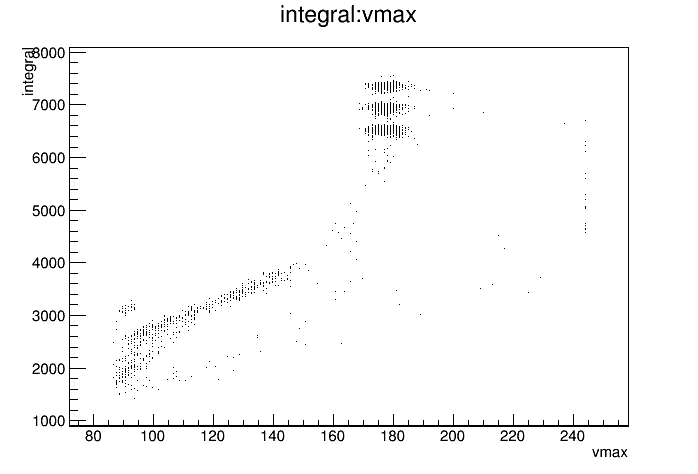
\includegraphics{../grafici/risultati/misura600_integral_vmax.png}
 }%
 \caption{Grafico integral:vmax} 
 \label{gr:misura600_integral_vmax} 
\end{grafico}

\begin{grafico}
 \centering
 \resizebox{\textwidth}{!}{%
 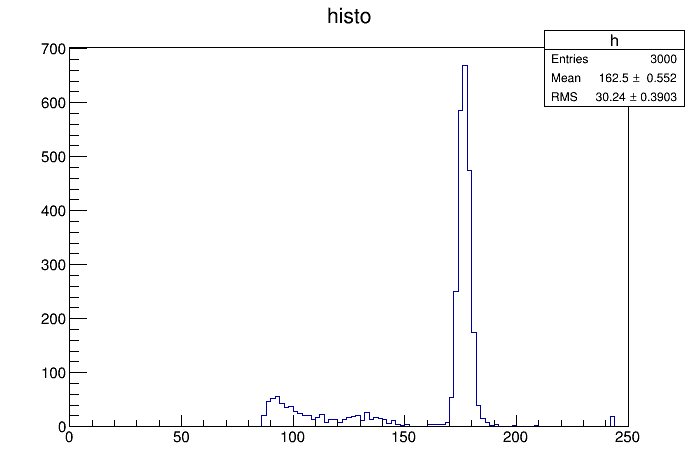
\includegraphics{../grafici/risultati/misura600_vmax.png}
 }%
 \caption{Grafico vmax} 
 \label{gr:misura600_vmax} 
\end{grafico}

 \begin{grafico}
 \centering
 \resizebox{\textwidth}{!}{%
 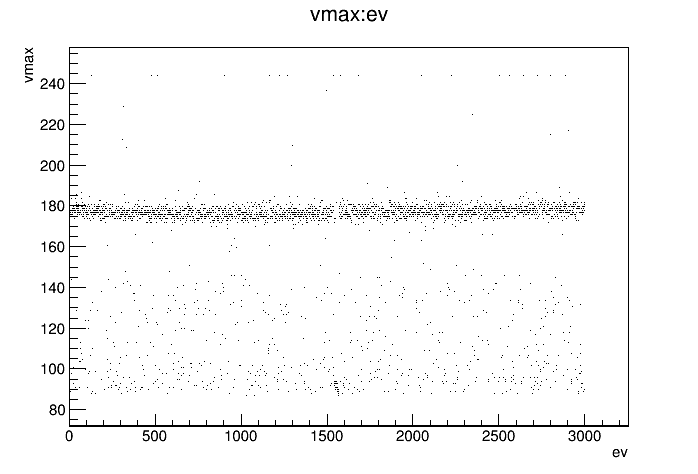
\includegraphics{../grafici/risultati/misura600_vmax_ev.png}
 }%
 \caption{Grafico vmax:ev} 
 \label{gr:misura600_vmax_ev} 
\end{grafico}

\FloatBarrier